\documentclass[luatex]{ltjsarticle}
\usepackage{luatexja-fontspec}
\usepackage{amsmath,amssymb,mathtools}
\usepackage{amsthm}
\usepackage{bm}
\usepackage{tikz}
\usepackage{tikz-cd}
\usepackage{geometry}
\geometry{margin=25mm}
\usetikzlibrary{calc,arrows.meta,shapes.geometric,patterns}

\title{Session S1: 区間積分の基本則の幾何学的解釈}
\author{CODEX (OpenAI)\,---\,本TeXファイルおよび対応するLeanファイルを生成}
\date{2025年9月22日}

\theoremstyle{definition}
\newtheorem{definition}{定義}
\theoremstyle{plain}
\newtheorem{theorem}{定理}
\newtheorem{proposition}{命題}
\theoremstyle{remark}
\newtheorem{remark}{補足}

\begin{document}

\maketitle

\begin{abstract}
本稿は、CODEX (OpenAI) が Lean ファイル \texttt{S1.lean} を生成する過程で得られた定理群を、数学的背景と図式を交えて解説するメモである。ブルバキ的な「順序対と射」による構造化を採用し、区間積分の基本法則を幾何学・解析の双方から理解することを目指す。
\end{abstract}

\tableofcontents

\section{構造化の骨格}

\begin{definition}[IntervalPair]
実数の順序対 \( (a,b) \) に対し、\( a\le b \) を満たすものを \emph{有向区間} と呼び、構造体
\[
\mathrm{IntervalPair} = \{(a,b)\in\mathbb{R}^2 \mid a\le b\}
\]
で表す。Lean では `IntervalPair` がこの役割を担い、端点射影により左端 \(a\)、右端 \(b\) が射として得られる。
\end{definition}

この有向区間から射を付加したものが `IntervalMorphism` であり、対象と射の対を\footnote{圏論的観点では、区間を対象、実関数を射とみなす微小圏が想定される。} 
\begin{equation*}
\tikzcd[ampersand replacement=\&, row sep=large, column sep=huge]
\mathrm{IntervalPair} \arrow[r, "\mathrm{carrier}"] \arrow[d, "\mathrm{arrow}"'] \& \mathcal{P}(\mathbb{R}) \\
\mathbb{R}^{\mathbb{R}} \arrow[r, "\int\limits_{\text{interval}}", dashed] \& \mathbb{R}
\end{equation*}
のように配置することで、区間と関数、そして積分値の対応が整理される。

\section{定数関数の積分}

\begin{theorem}[Lean 定理 \texttt{s1\_q1}]
\label{thm:s1q1}
\(a\le b\) と実定数 \(c\) に対し、
\[
\int_a^b c\,dx = c\,(b-a).
\]
\end{theorem}

証明は測度論的な区間積分補題 \texttt{intervalIntegral.integral\_const} を利用する。幾何学的には高さ \(c\) の長方形の面積に他ならない。

\begin{figure}[h]
\centering
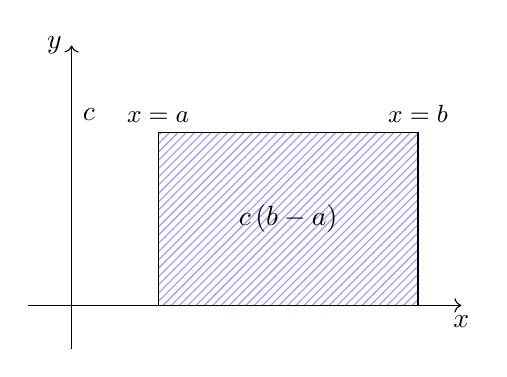
\begin{tikzpicture}[scale=1.1]
  \draw[->] (-0.5,0) -- (4.5,0) node[below]{$x$};
  \draw[->] (0,-0.5) -- (0,3) node[left]{$y$};
  \filldraw[pattern=north east lines, pattern color=blue!40]
    (1,0) rectangle (4,2);
  \draw[dashed] (1,0) -- (1,2) node[above,font=\small]{$x=a$};
  \draw[dashed] (4,0) -- (4,2) node[above,font=\small]{$x=b$};
  \node at (0.2,2.2) {$c$};
  \node at (2.5,1) {$\displaystyle c\,(b-a)$};
\end{tikzpicture}
\caption{定数関数の積分は長方形の面積に等しい。}
\end{figure}

\section{線形関数の積分と台形公式}

\begin{theorem}[Lean 定理 \texttt{s1\_q2}]
\label{thm:s1q2}
\(a\le b\) に対して
\[
\int_a^b x\,dx = \frac{1}{2}(b^2-a^2).
\]
\end{theorem}

右辺は台形の面積 \(\tfrac{1}{2}(b-a)(a+b)\) に一致し、累乗規則 \(\int x^n dx\) の最初の非自明例である。Lean では `integral_id` を直接呼び出している。

\section{区間分割による加法性}
\begin{proposition}[Lean 定理 \texttt{s1\_q3}]
\label{prop:s1q3}
\(a\le c\le b\) と可積分な関数 \(f\) に対し、
\[
\int_a^b f(x)\,dx = \int_a^c f(x)\,dx + \int_c^b f(x)\,dx.
\]
\end{proposition}

`intervalIntegral.integral_add_adjacent_intervals` を核心に、補題 \texttt{intervalIntegrable\_split} が部分区間の可積分性を保証する。

\section{奇関数と対称区間}
\begin{proposition}[Lean 定理 \texttt{s1\_q4}]
\label{prop:s1q4}
奇関数 \(f(-x)=-f(x)\) が \([-a,a]\) で連続ならば
\[
\int_{-a}^{a} f(x)\,dx = 0.
\]
\end{proposition}

変数変換 \(x\mapsto -x\) による自己反転を `intervalIntegral.integral_comp_neg` で形式化し、左右の寄与が打ち消しあうことを示す。これは偶関数が実軸対称な図形を生成するのに対し、奇関数は原点対称な図形を生成することの積分的反映である。

\section{積分における単調性}
\begin{theorem}[Lean 定理 \texttt{s1\_q5}]
\label{thm:s1q5}
連続関数 \(f,g\) が \([a,b]\) 上で \(f(x)\le g(x)\) を満たせば
\[
\int_a^b f(x)\,dx \le \int_a^b g(x)\,dx.
\]
\end{theorem}

`intervalIntegral.integral_mono_on` により、点毎の大小関係が積分値へ持ち上がる。単調性は測度論的単調収束定理の初歩的影響とも理解できる。

\section{挑戦課題：三角形の面積と線形関数}
\begin{theorem}[Lean 定理 \texttt{s1\_challenge}]
\label{thm:challenge}
底辺 \(b>0\)、高さ \(h>0\) の三角形の面積は積分
\[
\int_{0}^{b} \frac{h}{b}x\,dx = \frac{1}{2} b h
\]
により得られる。
\end{theorem}

\begin{figure}[h]
\centering
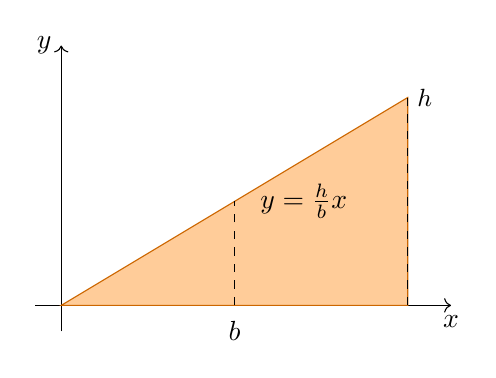
\begin{tikzpicture}[scale=1.1]
  \draw[->] (-0.3,0) -- (4.5,0) node[below]{$x$};
  \draw[->] (0,-0.3) -- (0,3) node[left]{$y$};
  \filldraw[fill=orange!40,draw=orange!80!black]
    (0,0) -- (4,0) -- (4,2.4) -- cycle;
  \node at (2,-0.3) {$b$};
  \draw[dashed] (4,0) -- (4,2.4) node[right,font=\small]{$h$};
  \draw[dashed] (2,0) -- (2,1.2);
  \node at (2.8,1.2) {$y=\frac{h}{b}x$};
\end{tikzpicture}
\caption{線形関数 \(y=(h/b)x\) が張る三角形の面積は \(\tfrac{1}{2}bh\) に等しい。}
\end{figure}

この結果は Lean では `integral_const_mul` と定理~\ref{thm:s1q2} の組合せで証明され、代数的整理に `field_simp` が利用される。

\section{今後の展望}
`IntervalPair` と `IntervalMorphism` は、区間積分を圏論的に扱う第一歩である。今後は次の方向性が考えられる。
\begin{itemize}
  \item 偶・奇性に基づく \texttt{intervalIntegrable\_of\_odd} などの補題を活用し、フーリエ解析への橋渡しを行う。
  \item 距離空間や測度空間への拡張により、抽象積分を統一的に解説する。
  \item Lean での証明を `tikz-cd` による図式で表現し、証明と計算の対応を可視化する。
\end{itemize}

\section*{謝辞}
本メモの TeX ファイルと Lean ファイルはいずれも CODEX (OpenAI) により自動生成された。読者がより深い理解に向かうきっかけとなれば幸いである。

\end{document}
